
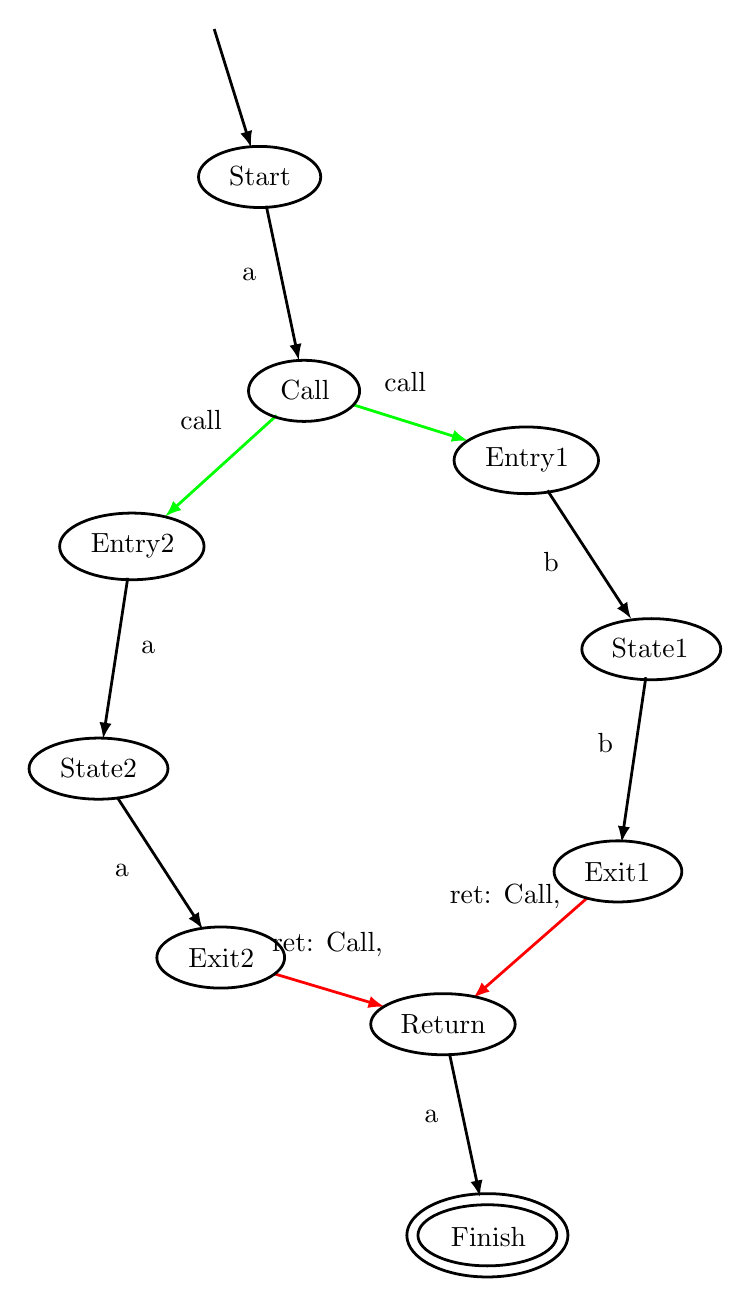
\begin{tikzpicture}[>=latex,line join=bevel,]
  \pgfsetlinewidth{1bp}
%%
\pgfsetcolor{black}
  % Edge: Exit2 -> Return
  \pgfsetcolor{red}
  \draw [->] (89.559bp,110.06bp) .. controls (98.492bp,107.39bp) and (109.32bp,104.16bp)  .. (128.97bp,98.288bp);
  \definecolor{strokecol}{rgb}{0.0,0.0,0.0};
  \pgfsetstrokecolor{strokecol}
  \draw (108.45bp,120.62bp) node {ret: Call, };
  % Edge: Call -> Entry1
  \pgfsetcolor{green}
  \draw [->] (117.69bp,314.99bp) .. controls (126.88bp,312.11bp) and (138.45bp,308.48bp)  .. (159bp,302.04bp);
  \definecolor{strokecol}{rgb}{0.0,0.0,0.0};
  \pgfsetstrokecolor{strokecol}
  \draw (136.41bp,323.06bp) node {call};
  % Edge: State2 -> Exit2
  \draw [->] (32.717bp,173.7bp) .. controls (39.406bp,163.38bp) and (49.826bp,147.31bp)  .. (63.446bp,126.3bp);
  \draw (34.352bp,147.21bp) node {a};
  % Edge: Exit1 -> Return
  \pgfsetcolor{red}
  \draw [->] (202.12bp,137.61bp) .. controls (193bp,129.6bp) and (179.63bp,117.88bp)  .. (160.98bp,101.53bp);
  \definecolor{strokecol}{rgb}{0.0,0.0,0.0};
  \pgfsetstrokecolor{strokecol}
  \draw (172.43bp,137.96bp) node {ret: Call, };
  % Edge: State1 -> Exit1
  \draw [->] (223.04bp,216.9bp) .. controls (221.21bp,204.49bp) and (218.13bp,183.55bp)  .. (214.3bp,157.45bp);
  \draw (208.43bp,193.35bp) node {b};
  % Edge: Start -> Call
  \draw [->] (86.401bp,386.61bp) .. controls (88.867bp,374.9bp) and (92.88bp,355.85bp)  .. (98.11bp,331.02bp);
  \draw (80.185bp,361.9bp) node {a};
  % Edge: Call -> Entry2
  \pgfsetcolor{green}
  \draw [->] (90.096bp,311.13bp) .. controls (81.318bp,303.17bp) and (68.434bp,291.49bp)  .. (50.037bp,274.81bp);
  \definecolor{strokecol}{rgb}{0.0,0.0,0.0};
  \pgfsetstrokecolor{strokecol}
  \draw (62.904bp,309.45bp) node {call};
  % Edge: Entry2 -> State2
  \draw [->] (36.531bp,252.69bp) .. controls (34.619bp,240.22bp) and (31.525bp,220.06bp)  .. (27.64bp,194.75bp);
  \draw (43.858bp,227.75bp) node {a};
  % Edge: Entry1 -> State1
  \draw [->] (187.62bp,284.15bp) .. controls (194.27bp,273.94bp) and (204.23bp,258.65bp)  .. (217.7bp,237.99bp);
  \draw (188.88bp,258.33bp) node {b};
  % Edge: Return -> Finish
  \draw [->] (152.36bp,81.346bp) .. controls (154.63bp,70.683bp) and (158.21bp,53.889bp)  .. (163.32bp,29.958bp);
  \draw (145.77bp,58.638bp) node {a};
  % Edge: Start__precursor__ -> Start
  \draw [->] (67.648bp,450.25bp) .. controls (70.757bp,440.27bp) and (74.64bp,427.81bp)  .. (80.911bp,407.69bp);
  % Node: Entry2
\begin{scope}
  \definecolor{strokecol}{rgb}{0.0,0.0,0.0};
  \pgfsetstrokecolor{strokecol}
  \draw (38bp,264bp) ellipse (26bp and 12bp);
  \draw (38.293bp,264.16bp) node {Entry2};
\end{scope}
  % Node: Finish
\begin{scope}
  \definecolor{strokecol}{rgb}{0.0,0.0,0.0};
  \pgfsetstrokecolor{strokecol}
  \draw (166bp,16bp) ellipse (25bp and 11bp);
  \draw (166bp,16bp) ellipse (29bp and 15bp);
  \draw (166.4bp,15.5bp) node {Finish};
\end{scope}
  % Node: Exit1
\begin{scope}
  \definecolor{strokecol}{rgb}{0.0,0.0,0.0};
  \pgfsetstrokecolor{strokecol}
  \draw (213bp,147bp) ellipse (23bp and 11bp);
  \draw (212.75bp,146.93bp) node {Exit1};
\end{scope}
  % Node: State2
\begin{scope}
  \definecolor{strokecol}{rgb}{0.0,0.0,0.0};
  \pgfsetstrokecolor{strokecol}
  \draw (26bp,184bp) ellipse (25bp and 11bp);
  \draw (26bp,184.06bp) node {State2};
\end{scope}
  % Node: Exit2
\begin{scope}
  \definecolor{strokecol}{rgb}{0.0,0.0,0.0};
  \pgfsetstrokecolor{strokecol}
  \draw (70bp,116bp) ellipse (23bp and 11bp);
  \draw (70.226bp,115.84bp) node {Exit2};
\end{scope}
  % Node: Start
\begin{scope}
  \definecolor{strokecol}{rgb}{0.0,0.0,0.0};
  \pgfsetstrokecolor{strokecol}
  \draw (84bp,397bp) ellipse (22bp and 11bp);
  \draw (84.15bp,397.3bp) node {Start};
\end{scope}
  % Node: State1
\begin{scope}
  \definecolor{strokecol}{rgb}{0.0,0.0,0.0};
  \pgfsetstrokecolor{strokecol}
  \draw (225bp,227bp) ellipse (25bp and 11bp);
  \draw (224.58bp,227.43bp) node {State1};
\end{scope}
  % Node: Entry1
\begin{scope}
  \definecolor{strokecol}{rgb}{0.0,0.0,0.0};
  \pgfsetstrokecolor{strokecol}
  \draw (180bp,295bp) ellipse (26bp and 12bp);
  \draw (180.3bp,295.36bp) node {Entry1};
\end{scope}
  % Node: Call
\begin{scope}
  \definecolor{strokecol}{rgb}{0.0,0.0,0.0};
  \pgfsetstrokecolor{strokecol}
  \draw (100bp,320bp) ellipse (20bp and 11bp);
  \draw (100.34bp,320.42bp) node {Call};
\end{scope}
  % Node: Return
\begin{scope}
  \definecolor{strokecol}{rgb}{0.0,0.0,0.0};
  \pgfsetstrokecolor{strokecol}
  \draw (150bp,92bp) ellipse (26bp and 11bp);
  \draw (150.09bp,91.98bp) node {Return};
\end{scope}
%
\end{tikzpicture}
